\section{函数的基本性质}

\begin{theorem}[常见的奇偶函数]
    \begin{itemize}
        \item     常见奇函数：$x^{2 n+1}, \sin x, \tan x, \arcsin x, \arctan x, \ln \frac{1-x}{1+x}, \ln \left(x+\sqrt{1+x^2}\right) \ldots$
        \item     常见偶函数：$C, x^{2 n},|x|, \cos x, \mathrm{e}^x+\mathrm{e}^{-x} \cdot \cdots$
    \end{itemize}
\end{theorem}

\subsection{反双曲正弦函数}

\begin{theorem}[反双曲正弦函数]
    $$\ln \left(x+\sqrt{1+x^2}\right)$$
    $$
        \begin{aligned}
             & \left\{\begin{array}{l}
                          \text { (1) 奇 }                                                       \\
                          \text { (2) } \ln \left(x+\sqrt{1+x^2}\right) \sim x, x \rightarrow 0 \\
                          \text { (3) }\left[\ln \left(x+\sqrt{1+x^2}\right)\right]^{\prime}=\frac{1}{\sqrt{1+x^2}}
                      \end{array}\right.
        \end{aligned}
    $$
\end{theorem}

\begin{theorem}
    事实上，任何一个定义域关于原点对称的函数都可以看成奇函数和偶函数之和。$y=f(x)$ 的定义域关于原点对称，则：
    \begin{itemize}
        \item $F(x)=\frac{f(x)+f(-x)}{2}$ 为偶函数；
        \item $G(x)=\frac{f(x)-f(-x)}{2}$ 为奇函数；
        \item 且 $f(x)=F(x)+G(x)$ ．
    \end{itemize}
\end{theorem}

\begin{theorem}[复合函数的奇偶性]
    内偶则偶，内奇同外。例如 $\ln \left(\sin x+\sqrt{1+\sin ^2 x}\right)$ 是奇函数。
\end{theorem}

\begin{theorem}[求导的奇偶性]
    $f(x)$ 若是奇函数，求导后一定会变成偶函数。反之亦然。
\end{theorem}

\subsection{周期函数的性质}

\begin{theorem}[周期函数的性质]
    \begin{enumerate}
        \item  $\sin x, \cos x$ 以 $2 \pi$ 为周期；
        \item  $\tan x, \cot x,|\tan x|,|\cot x|,|\sin x|,|\cos x|$ 以 $\pi$ 为周期；
        \item 若 $f(x)$ 以 $T$ 为周期，则 $f(a x+b)$ 以 $\frac{T}{|a|}$ 为周期 $(a \neq 0)$ ；
        \item 若 $f(x), g(x)$ 分别以 $T_1, T_2$ 为周期，且 $T_1 / T_2$ 为有理数，则 $f(x) \pm g(x)$ 和 $f(x) g(x)$也是周期函数，其一个周期为 $T_1, T_2$ 的最小公倍数；
    \end{enumerate}
\end{theorem}

\begin{example}
    $
        \begin{gathered}
            \sin \left(-3 x+\frac{\pi}{3}\right) \cos 2 x
        \end{gathered}
    $ 这个函数是以 $2\pi$ 为周期的。因为第一个周期是 $\frac{2\pi}{3}$，最小公倍周期为 $2\pi$.
\end{example}

\section{对数函数常用运算性质}

\begin{example}
    $$
        \begin{aligned}
             & (\sin x)^x=e^{x \ln \sin x}                         \\
             & (1+x)^{\frac{1}{x}}=e^{\frac{1}{x} \times \ln(1+x)}
        \end{aligned}
    $$
\end{example}

\section{三角函数的正割和余割}

\begin{definition}[正割函数]
    形如$y=\sec x = \frac{1}{\cos x}$的函数称为正割函数。
\end{definition}

\begin{definition}[余割函数]
    形如$y=\csc x = \frac{1}{\sin x}$的函数称为余割函数。
\end{definition}

\begin{tips}
    哈哈，正割居然是余弦的倒数。
\end{tips}

\section{讨论式的诱导公式}

\begin{theorem}
    \begin{itemize}
        \item     $\sin (\alpha \pm n \pi)=(-1)^n \sin \alpha$.
        \item     $\sin (n \pi-\alpha)=(-1)^{n+1} \sin \alpha$.
    \end{itemize}
\end{theorem}

\section{和差化积和积化和差}

\begin{theorem}
    $$
        \begin{array}{ll}
            \cos \alpha \cos \beta=\frac{1}{2}[\cos (\alpha+\beta)+\cos (\alpha-\beta)] & \sin \alpha \sin \beta=-\frac{1}{2}[\cos (\alpha+\beta)-\cos (\alpha-\beta) \\
            \sin \alpha \cos \beta=\frac{1}{2}[\sin (\alpha+\beta)+\sin (\alpha-\beta)] & \cos \alpha \sin \beta=\frac{1}{2}[\sin (\alpha+\beta)-\sin (\alpha-\beta)
        \end{array}
    $$
    注：积化和差公式的证明可以直接将右边展开得到左边．
    $$
        \begin{array}{ll}
            \sin x+\sin y=2 \sin \frac{x+y}{2} \cos \frac{x-y}{2} & \sin x-\sin y=2 \cos \frac{x+y}{2} \sin \frac{x-y}{2}  \\
            \cos x+\cos y=2 \cos \frac{x+y}{2} \cos \frac{x-y}{2} & \cos x-\cos y=-2 \sin \frac{x+y}{2} \sin \frac{x-y}{2}
        \end{array}
    $$
\end{theorem}

\section{平方关系}

\begin{theorem}
    $$\sin ^2 \alpha+\cos ^2 \alpha=1 ; 1+\tan ^2 \alpha=\sec ^2 \alpha ; 1+\cot ^2 \alpha=\csc ^2 \alpha$$
\end{theorem}

\subsection{六边形记忆法}

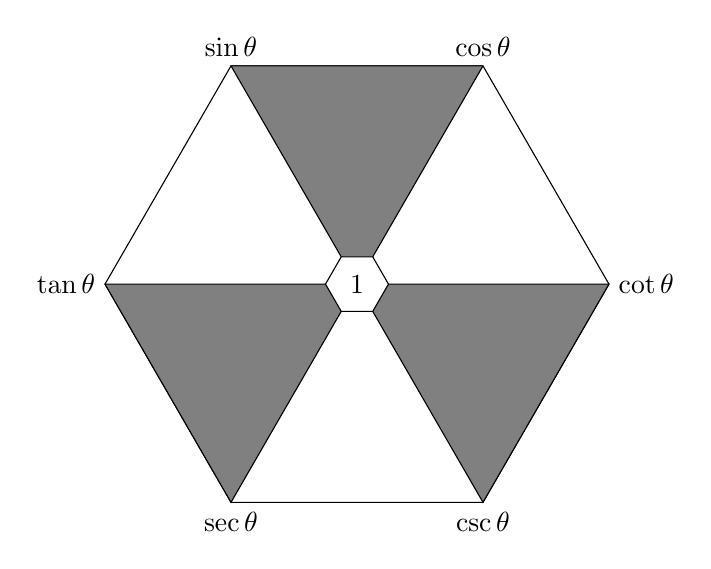
\begin{tikzpicture}[scale=4,cap=round,>=latex]
    % Radius of regular polygons
    \newdimen\R
    \R=0.8cm
    \coordinate (center) at (0,0);
    \draw (0:\R)
    \foreach \x in {60,120,...,360} {  -- (\x:\R) }
    -- cycle (300:\R) node[below] {$\csc \theta$}
    -- cycle (240:\R) node[below] {$\sec \theta$}
    -- cycle (180:\R) node[left] {$\tan \theta$}
    -- cycle (120:\R) node[above] {$\sin \theta$}
    -- cycle (60:\R) node[above] {$\cos \theta$}
    -- cycle (0:\R) node[right] {$\cot \theta$};
    \draw { (60:\R) -- (120:\R) -- (center) -- (60:\R) } [fill=gray];
    \draw { (180:\R) -- (240:\R) -- (center) -- (180:\R) } [fill=gray];
    \draw { (0:\R) -- (300:\R) -- (center) -- (0:\R) }  [fill=gray];
    \R=0.1cm
    \draw (0:\R) \foreach \x in {60,120,...,360} { -- (\x:\R) }
        [fill=white] -- cycle (center) node {1};
\end{tikzpicture}

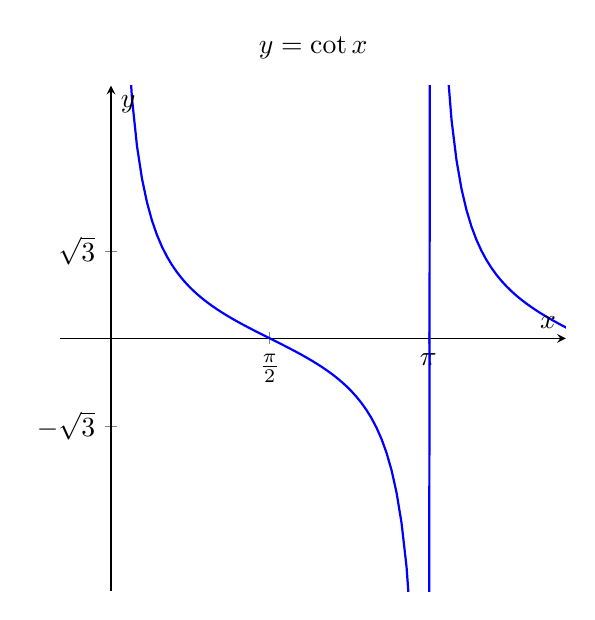
\begin{tikzpicture}
    \begin{axis}[
            title={$y=\cot x$},
            axis lines=middle,
            xlabel={$x$},
            ylabel={$y$},
            xmin=-0.5, xmax=4.5,
            ymin=-5, ymax=5,
            xtick={0, 1.57, 3.14},
            xticklabels={0, $\frac{\pi}{2}$, $\pi$},
            ytick={-1.732, 1.732},
            yticklabels={$-\sqrt{3}$, $\sqrt{3}$},
            domain=0.01:4.9, % 设置绘图域以避开奇点
            samples=100,
            unbounded coords=jump, % 遇到奇点时断开曲线
            width=8cm, height=8cm,
        ]
        \addplot[blue, thick] {1/tan(deg(x))};
    \end{axis}
\end{tikzpicture}

\pgfmathdeclarefunction{acot}{1}{%
    \pgfmathparse{pi/2 - atan(#1)}%
}

\begin{tikzpicture}
    \begin{axis}[
            title={$y=\operatorname{arccot} x$},
            axis lines=middle,
            xlabel={$x$},
            ylabel={$y$},
            xmin=-5, xmax=5,
            ymin=-0.5, ymax=3.5,
            xtick={0},
            xticklabels={0},
            ytick={0, 1.57, 3.14},
            yticklabels={0, $\frac{\pi}{2}$, $\pi$},
            domain=-5:5,
            samples=100,
            width=8cm, height=8cm,
        ]
        \addplot[red, thick] {rad(acot(x))};
        % 绘制渐近线
        \addplot[dashed, domain=-5:5] {pi};
        \addplot[dashed, domain=-5:5] {0};
    \end{axis}
\end{tikzpicture}
